\chapter{ZweiteErfahrung} \label{cha:ZweiteErfahrung}

In diesem Kapitel wird der durch die Projektgruppe implementierte VXI-11-Server vorgestellt und in den einzelnen Abschnitten auf die Teilbereiche Hardware, Software und auf Kommunikationsschnittstellen mit Test- und Messgeräten eingegangen. Die grundlegende Idee des VXI-11-Servers ist die Kommunikation mit Geräten über Ethernet, welche unterschiedliche Kommunikationsstandards nutzen. Hierzu ist eine entsprechende Hardware notwendig, um verschiedenste Kommunikationsstandards anschließen zu können und eine entsprechende softwaretechnische Implementierung. Auf die Realisierung dieser Teilbereiche wird im folgenden eingegangen.

\section{Grundlegende Einführung} 
\cite{lin1973}.

\section{Bildregistrierung} 

\begin{figure}[htb]
 \centering 
 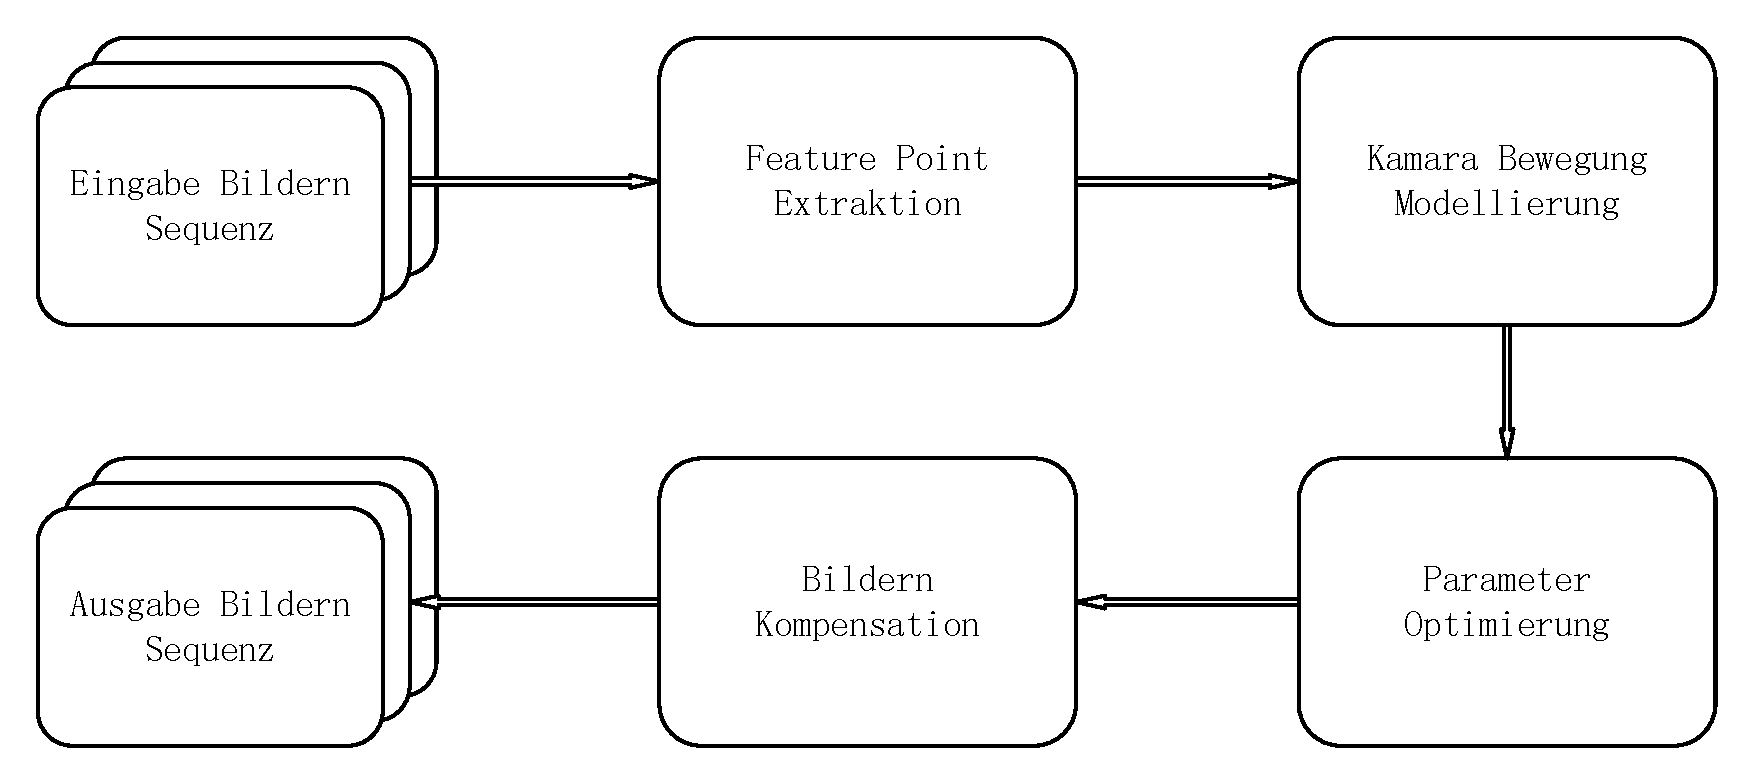
\includegraphics[keepaspectratio,width=0.8\textwidth]{images/0_Image_Registration_Flussdiagramm.pdf}
 \caption{Flussdiagramm der Bildregistrierung}
 \label{fig:Bildregistrierung}
\end{figure}

\subsection{SURF}
Hier wird zuerste die SURF\cite{Surf} Feature Detektion eingegangen. Der SURF-Algorithmus arbeitet mit integrierten Bildern. Die Faltung bezieht sich nur auf das vorherige Bild, und mit Erhöhung der Größe des Bildkerns können das Heruntertaktung-Verfahren realisiert werden. 

\textbf{Algorithmus:}\\
\\
$\bullet$ \textbf{Aufbau einer hessischen Matrix.}\\
Die Hesse-Matrix stellt den Kern des SURF-Algorithmus dar. Zur Vereinfachung der Operation wird die Funktion f (z, y) angenommen, dass die Hesse-Matrix H setzt sich aus Funktionen und partiellen Ableitungen zusammen:

\begin{equation}
   \mathcal{H}(f(x,y)) = \begin{bmatrix}
   \frac{\partial^{2}f}{\partial x^{2}} & \frac{\partial^{2}f}{\partial x \cdot \partial y} \\
   \frac{\partial^{2}f}{\partial x \cdot \partial y} & \frac{\partial^{2}f}{\partial y^{2}} \\   
   \end{bmatrix}
\end{equation}

 Diskriminante der H-Matrix läuft:
 
\begin{equation}
   \det(\mathcal{H}) = \frac{\partial^{2}f}{\partial x^{2}} \cdot \frac{\partial^{2}f}{\partial y^{2}} - (\frac{\partial^{2}f}{\partial x \cdot \partial y})^2  
\end{equation}

Der Wert der Diskriminante ist der Eigenwert der H-Matrix. Durch dessen positiven und negativen wird bestimmt, ob der Punkt ein Extrempunkt ist oder nicht. Im SURF Algorithmus wird das Bildpixel $l(x,y)$ anstelle des Funktionswertes $f(x,y)$ verwendet. Nutzen eine Zweite-Order Gaussian function als Filter. Die zweiten Partielle Ableitungen können durch Faltung zwischen bestimmten Kernen berechnet werden. Dadurch können die Werte der drei Matrixelemente der H-Matrix berechnet werden, d.h. die H-Matrix berechnet:

\begin{equation}
\begin{split}
   &\mathcal{H}(\textbf{x},\sigma) = \begin{bmatrix}
   L_{xx}(\textbf{x},\sigma)\ L_{xy}(\textbf{x},\sigma) \\
   L_{xy}(\textbf{x},\sigma)\ L_{yy}(\textbf{x},\sigma)
   \end{bmatrix} \\   
   &L(\textbf{x},\sigma) = G(\sigma)*I(\textbf{x}) \\  
   &G(\sigma) = \frac{\partial^{2}g(\sigma)}{\partial x^{2}}      
\end{split}
\end{equation}


Hier $L_{xx}(\textbf{x},\sigma)$ bedeutet die Faltung der zweiter Gaussian Ableitung $G(\sigma)$ mit dem Bild I in Punkt $\textbf{x}$(x,y), ähnlich für $L_{xy}(\textbf{x},\sigma)$ und $L_{yy}(\textbf{x},\sigma)$. Auf diese Weise kann der Wert der Determinante für jedes Pixel in dem Bild berechnet werden, und dieser Wert kann verwendet werden, um den Merkmalspunkt zu feststellen.
Zur einfacheren Anwendung schlägt Herbert Bay\cite{Surf} vor, L mit einer Approximation ersetzen. Um den Fehler zwischen dem genauen Wert und der Approximation auszugleichen, kann die H-Matrix-Diskriminante wie folgt ausgedrückt werden:

\begin{equation}
   \det(\mathcal{H}_{Approx}) = D_{xx}D_{yy} - (0.9D_{xy})^2  
\end{equation}
\\
$\bullet$ \textbf{Erstellen Maßstab Raum}\\
Der Maßstabsraum $L(\textbf{x},\sigma)$ des Bildes ist die Darstellung dieses Bildes bei unterschiedlichen Auflösungen(Skalierung). Im Bereich der Computer Vision wird der Maßstabsraum symbolisch als Bildpyramide ausgedrückt. Wobei die Eingangsbildfunktion wiederholt mit dem Kern der Gaußschen Funktion gefaltet und wiederholt unterabgetastet wird.Diese Methode wird hauptsächlich für die Implementierung des SIFT Algorithmus verwendet. Jede Bildschicht hängt jedoch von der vorherigen Bildschicht ab, und das Bild muss in der Größe angepasst werden.Daher hat diese Berechnungsmethode eine große Kosten in Berechnung. Dagegen in SURF Algorithmus, die Verfahre ist durch die Erhöhung der Größe des Bildkerns. Diese ist auch der Unterschied zwischen dem SIFT Algorithmus und dem SURF Algorithmus bei der Verwendung des Pyramidenprinzips.
Der Algorithmus ermöglicht, dass mehrere Bilder des Maßstabsraums gleichzeitig verarbeitet werden, ohne dass das Bild unterabgetastet wird, wodurch die Leistung des Algorithmus verbessert wird. Das linke Bild in Abbildung 4.2 ist eine Pyramidenstruktur, die auf herkömmliche Weise erstellt wird, die Größe des Bildes wird geändert, und die Operation wird die Unterebene  unter Verwendung der Gaußschen Funktion wiederholt glätten. Der Surf Algorithmus auf der rechten Seite in Abbildung 4.2 behält das ursprüngliche Bild unverändert und ändert nur die Filtergröße.

\begin{figure}[htb]
 \centering 
 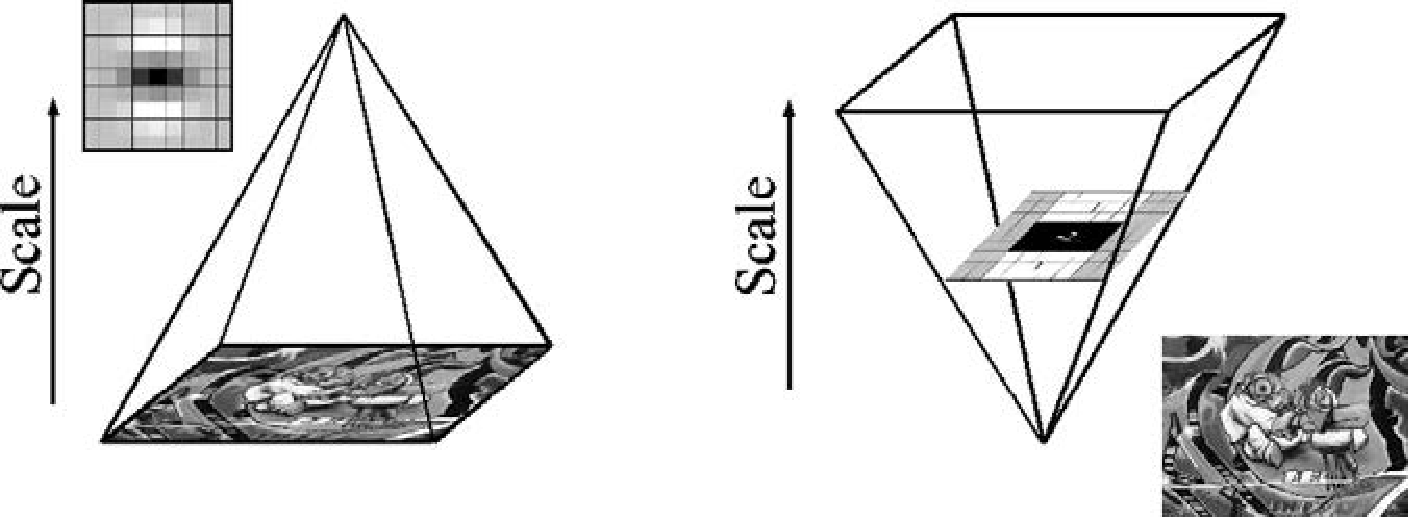
\includegraphics[keepaspectratio,width=0.8\textwidth]{images/4_ZweiteErfahrung/Pyramidenstruktur.pdf}
 \caption{Scale space}
 \label{fig:Scale space}
\end{figure} 


$\bullet$ \textbf{Präzise Lokalisierung von Feature-Punkten}\\
Vergleichen die Größe jedes Pixel, das von der hessischen Matrix verarbeitet wird, mit 26 Punkten in seiner drei Dimensionen Raum.

\subsection{RANSAC}

\subsection{Kamara Model}

\subsection{Parameter Optimierung}

\section{Differenzbild}


\section{Image Processing} 


\section{QR Pattern Detection} 


Nicht vergessen, dass Überschriften nicht aufeinander folgen dürfen\ldots

\begin{otherlanguage}{english}
\section{TexLipse spell checking}
%
To enable spell checking in TeXLipse, download the respective dictionaries from 
\url{https://sourceforge.net/projects/texlipse/files/dictionaries/}.

Save the dictionaries at a local location and enter the path in \texttt{Window->Preferences->Tex\-lipse->Spell Checker} (see Fig. \ref{fig:dict_path}).
%
\begin{figure}[htb]
	\centering
	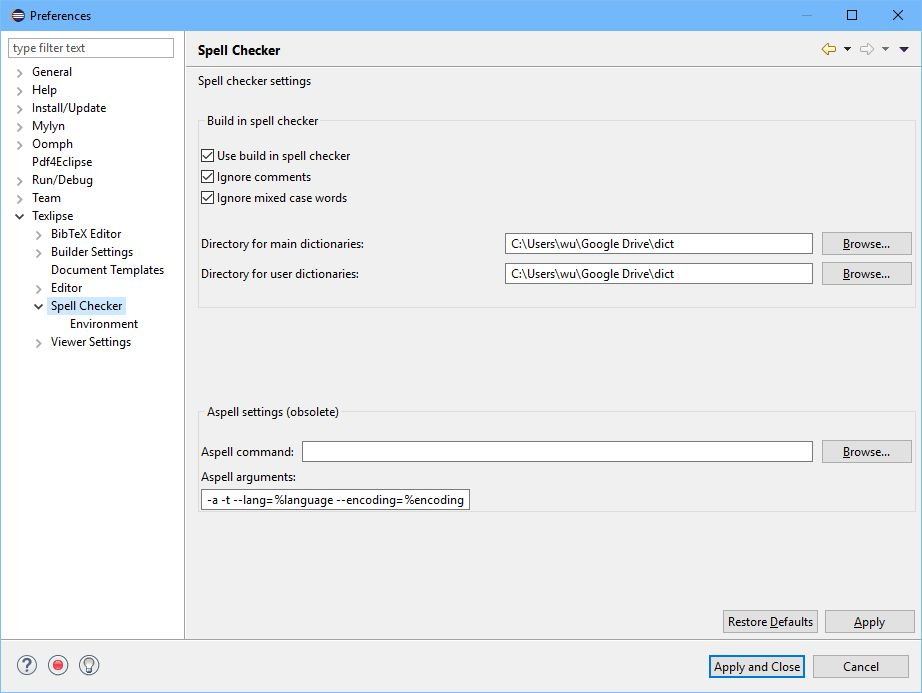
\includegraphics[scale=0.40]{images/Spell_Checker_preferences.jpg}
	\captionbelow{TeXLipse Spell Checker preferences}
	\label{fig:dict_path}
\end{figure}

To synchronize the user dictionaries between multiple machines, it might be useful to save the dictionaries in your google drive or drop box.

\section{Enable tikzexternalize for PdfLatex}

Go to \texttt{Window->Preferences->Texlipse->Builder Settings} and add 
%
\begin{verbatim}
--shell-escape
\end{verbatim}
%
to the command arguments (see Fig. \ref{fig:builder_settings}).
%
\begin{figure}[htb]
	\centering
	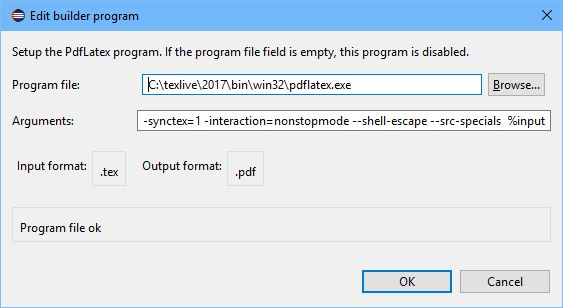
\includegraphics[scale=0.40]{images/PdfLatex_settings.jpg}
	\captionbelow{PdfLatex Builder Settings}
	\label{fig:builder_settings}
\end{figure}

\section{Forward search with TeXlipse and Sumatra PDF}

Download and install SumatraPDF: \url{https://www.sumatrapdfreader.org/}.

Then edit the viewer settings for SumatraPDF in \texttt{Window->Preferences->Texlipse->Viewer Settings}.

Change the viewer arguments to
%
\begin{verbatim}
-reuse-instance %fullfile -forward-search %texfile %line
\end{verbatim}
%
and leave all DDE message field empty.
Change the inverse search support to "`Viewer runs external command"' and enable "`Viewer supports forward search"'.

Figure \ref{fig:viewer_settings} displays the dialog window.
%
\begin{figure}[htb]
	\centering
	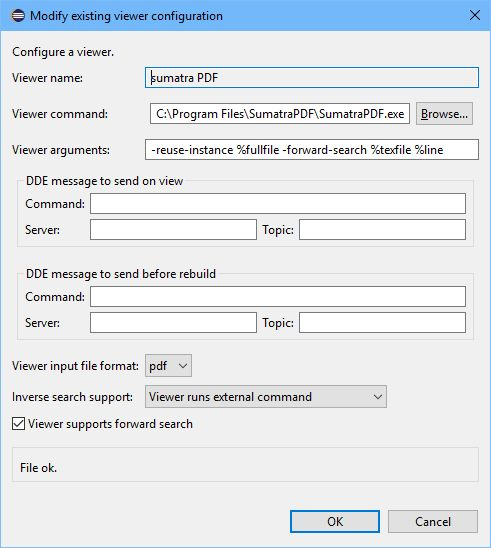
\includegraphics[scale=0.40]{images/Viewer_settings.jpg}
	\captionbelow{TeXLipse Viewer Settings}
	\label{fig:viewer_settings}
\end{figure}

In SumatraPDF configure the inverse search command via the \texttt{Settings->Options} menu (see Fig. \ref{fig:sumatrapdf_options}).
%
\begin{figure}[htb]
	\centering
	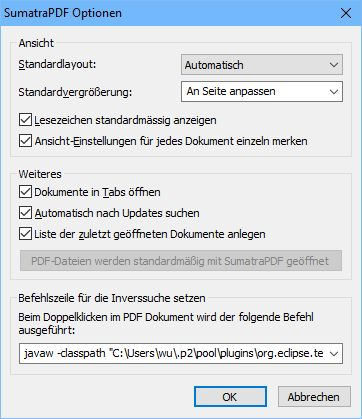
\includegraphics[scale=0.40]{images/SumatraPDF_optionen.jpg}
	\captionbelow{SumatraPDF Options}
	\label{fig:sumatrapdf_options}
\end{figure}

If you have install TeXlipse~1.5.0, the inverse search command will look like this:

\begin{lstlisting}[breaklines=true, basicstyle=\ttfamily, columns=flexible]
javaw -classpath "C:\Users\wu\.p2\pool\plugins\net.sourceforge.texlipse_1.5.0\texlipse.jar" net.sourceforge.texlipse.viewer.util.FileLocationClient -p 55000 -f "%f" -l %l
\end{lstlisting}

Let the path point to your eclipse share pool. Or if you do not have a shared pool, choose the plugins directory of your eclipse installation.

For TeXLipse~2.0.X the FileLocationClient is relocated to org.eclipse.texlipse making the inverse search command look like the following.
\begin{lstlisting}[breaklines=true, basicstyle=\ttfamily, columns=flexible]
javaw -classpath "C:\Users\wu\.p2\pool\plugins\org.eclipse.texlipse_2.0.1.201801202105\texlipse.jar" org.eclipse.texlipse.viewer.util.FileLocationClient -p 55000 -f "%f" -l %l
\end{lstlisting}

\end{otherlanguage}